\documentclass[tikz, border=5mm]{standalone}
\usepackage{tikz}

\begin{document}

% n=4 GT-pattern: left-interlacing positions and transpositions
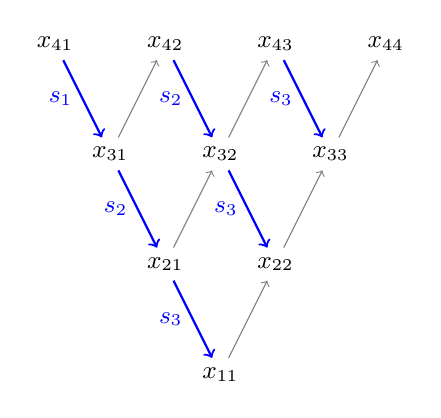
\begin{tikzpicture}[scale=1.4, every node/.style={font=\small}]
% Row 4 (top): lambda
\node (x41) at (0, 3) {$x_{41}$};
\node (x42) at (1, 3) {$x_{42}$};
\node (x43) at (2, 3) {$x_{43}$};
\node (x44) at (3, 3) {$x_{44}$};
% Row 3
\node (x31) at (0.5, 2) {$x_{31}$};
\node (x32) at (1.5, 2) {$x_{32}$};
\node (x33) at (2.5, 2) {$x_{33}$};
% Row 2
\node (x21) at (1.0, 1) {$x_{21}$};
\node (x22) at (2.0, 1) {$x_{22}$};
% Row 1
\node (x11) at (1.5, 0) {$x_{11}$};

% Left interlacing edges with transposition labels
\draw[->, thick, blue] (x41) -- (x31) node[midway, left] {$s_1$};
\draw[->, thick, blue] (x42) -- (x32) node[midway, left] {$s_2$};
\draw[->, thick, blue] (x43) -- (x33) node[midway, left] {$s_3$};
\draw[->, thick, blue] (x31) -- (x21) node[midway, left] {$s_2$};
\draw[->, thick, blue] (x32) -- (x22) node[midway, left] {$s_3$};
\draw[->, thick, blue] (x21) -- (x11) node[midway, left] {$s_3$};

% Right interlacing edges (thin, grey, no labels)
\draw[->, thin, gray] (x31) -- (x42);
\draw[->, thin, gray] (x32) -- (x43);
\draw[->, thin, gray] (x33) -- (x44);
\draw[->, thin, gray] (x21) -- (x32);
\draw[->, thin, gray] (x22) -- (x33);
\draw[->, thin, gray] (x11) -- (x22);
\end{tikzpicture}

% n=3 GT-pattern: left-interlacing positions and transpositions
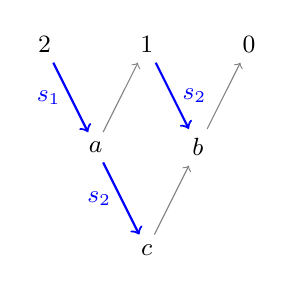
\begin{tikzpicture}[scale=1.3, every node/.style={font=\small}]
\node (x31) at (0, 2) {$2$};
\node (x32) at (1, 2) {$1$};
\node (x33) at (2, 2) {$0$};
\node (x21) at (0.5, 1) {$a$};
\node (x22) at (1.5, 1) {$b$};
\node (x11) at (1.0, 0) {$c$};

\draw[->, thick, blue] (x31) -- (x21) node[midway, left] {$s_1$};
\draw[->, thick, blue] (x32) -- (x22) node[midway, right] {$s_2$};
\draw[->, thick, blue] (x21) -- (x11) node[midway, left] {$s_2$};

\draw[->, thin, gray] (x21) -- (x32);
\draw[->, thin, gray] (x22) -- (x33);
\draw[->, thin, gray] (x11) -- (x22);
\end{tikzpicture}

\end{document}
